% ============================================================================
%  Figure 1 - processing timeline of a compound truck and the outbound truck
%             of its retained destination.
%  Target: Journal of the Korean Institute of Industrial Engineers (JKIIE)
%
%  Build :  xelatex fig0_compound_timeline.tex      (pdflatex also works)
%  Output:  fig0_compound_timeline.pdf
%
%  Drawn at FINAL PRINT SIZE (145 x 57 mm) so that it is included at natural
%  size and never rescaled.  Labels are therefore true 8 pt / 9 pt, matching
%  the 10 pt body font of jkiie_submit_body.tex.
%
%  In the paper, include it WITHOUT a width option:
%      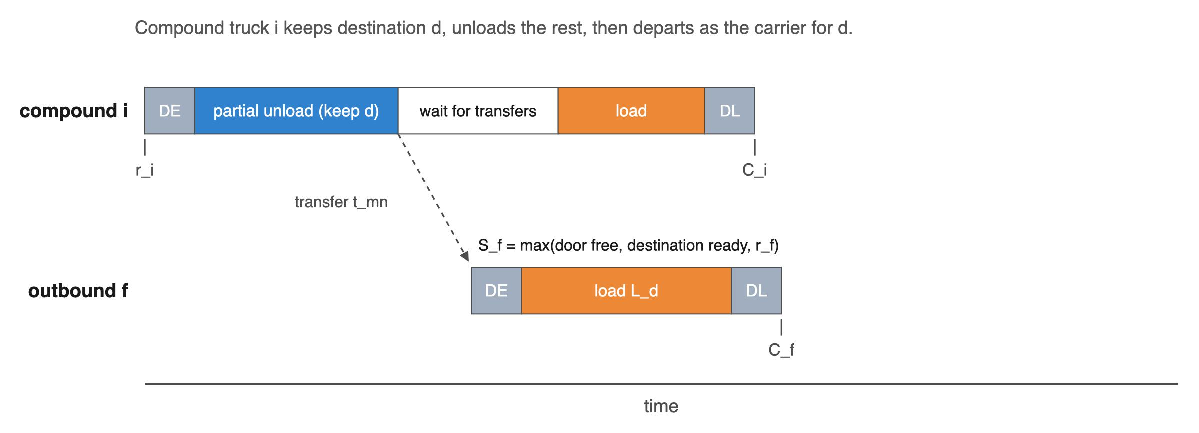
\includegraphics{fig0_compound_timeline.pdf}
% ============================================================================
\documentclass[10pt,border=2pt]{standalone}
\usepackage{tikz}
\usepackage{amsmath}
\usetikzlibrary{arrows.meta}

% ---- palette ---------------------------------------------------------------
% JKIIE prints some issues in grayscale; flip this switch for a B&W-safe
% version with well-separated lightness values (0.45 / 0.65 / 0.85 / white).
\newif\ifgrayfig
\grayfigfalse                     % <- \grayfigtrue for grayscale

\ifgrayfig
  \definecolor{cDoor}  {gray}{0.45}
  \definecolor{cUnload}{gray}{0.65}
  \definecolor{cLoad}  {gray}{0.85}
  \colorlet{tDoor}{white}\colorlet{tUnload}{black}\colorlet{tLoad}{black}
\else
  \definecolor{cDoor}  {HTML}{A0AEC0}
  \definecolor{cUnload}{HTML}{3182CE}
  \definecolor{cLoad}  {HTML}{ED8936}
  \colorlet{tDoor}{white}\colorlet{tUnload}{white}\colorlet{tLoad}{white}
\fi
\definecolor{ink} {HTML}{1A1A1A}
\definecolor{axis}{HTML}{4D4D4D}

% ---- one door-occupancy block ----------------------------------------------
% #1 x   #2 width   #3 y-centre   #4 fill   #5 text colour   #6 label
\newcommand{\dockbar}[6]{%
  \draw[blk,fill=#4] ({#1},{#3-4}) rectangle ({#1+#2},{#3+4});%
  \node[font=\footnotesize,text=#5,inner sep=0pt] at ({#1+#2/2},{#3}) {#6};%
}

\begin{document}
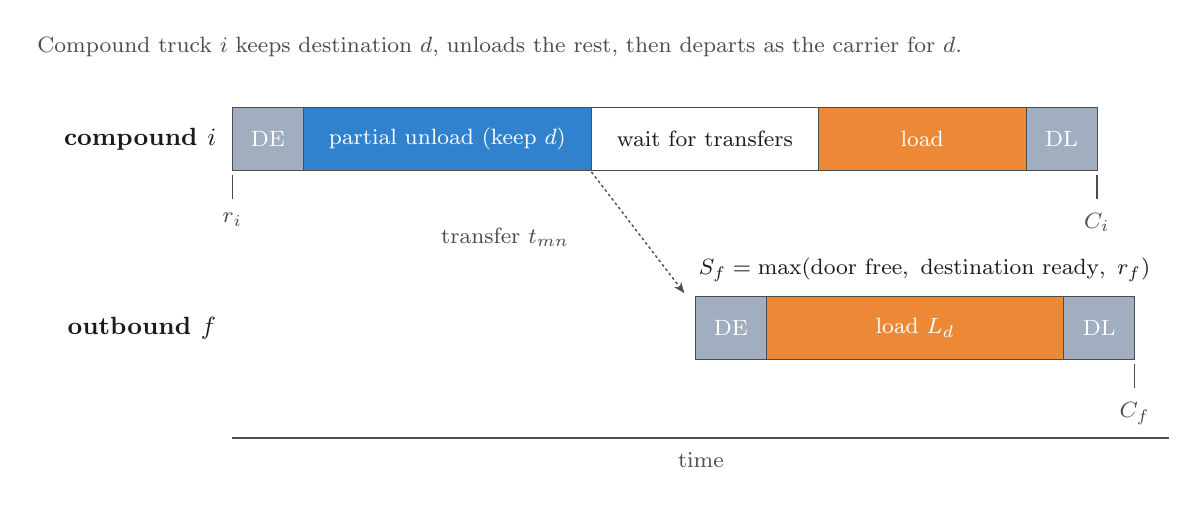
\begin{tikzpicture}[x=1mm,y=1mm,
    blk/.style ={draw=axis,line width=0.3pt},
    tick/.style={draw=axis,line width=0.4pt},
  ]

% fixed bounding box -> figure width stays stable across edits
\path (0,4) rectangle (145,-53);

% ---- headnote --------------------------------------------------------------
\node[anchor=base west,font=\footnotesize,text=axis] at (0,1)
  {Compound truck $i$ keeps destination $d$, unloads the rest,
   then departs as the carrier for $d$.};

% ---- compound truck i ------------------------------------------------------
\node[anchor=east,font=\small\bfseries,text=ink,inner sep=0pt]
  at (24,-10) {compound $i$};

\dockbar{26}   {9}   {-10}{cDoor} {tDoor} {DE}
\dockbar{35}   {36.6}{-10}{cUnload}{tUnload}{partial unload (keep $d$)}
\dockbar{71.6} {28.8}{-10}{white} {ink}   {wait for transfers}
\dockbar{100.4}{26.4}{-10}{cLoad} {tLoad} {load}
\dockbar{126.8}{9}   {-10}{cDoor} {tDoor} {DL}

\draw[tick] (26,-14.6) -- (26,-17.6);
\node[anchor=north,font=\footnotesize,text=axis] at (26,-18.2) {$r_i$};
\draw[tick] (135.8,-14.6) -- (135.8,-17.6);
\node[anchor=north,font=\footnotesize,text=axis] at (135.8,-18.2) {$C_i$};

% ---- outbound truck f ------------------------------------------------------
\node[anchor=east,font=\small\bfseries,text=ink,inner sep=0pt]
  at (24,-34) {outbound $f$};

\node[anchor=south west,font=\footnotesize,text=ink] at (84,-29.4)
  {$S_f=\max(\text{door free},\ \text{destination ready},\ r_f)$};

\dockbar{84.8} {9}   {-34}{cDoor}{tDoor}{DE}
\dockbar{93.8} {37.8}{-34}{cLoad}{tLoad}{load $L_d$}
\dockbar{131.6}{9}   {-34}{cDoor}{tDoor}{DL}

\draw[tick] (140.6,-38.6) -- (140.6,-41.6);
\node[anchor=north,font=\footnotesize,text=axis] at (140.6,-42.2) {$C_f$};

% ---- transfer dependency ---------------------------------------------------
\draw[axis,line width=0.5pt,dash pattern=on 1pt off 1pt,
      -{Stealth[length=1.4mm,width=1.1mm]}] (71.6,-14.2) -- (83.4,-29.6);
\node[anchor=east,font=\footnotesize,text=axis] at (70,-22.5)
  {transfer $t_{mn}$};

% ---- time axis -------------------------------------------------------------
\draw[axis,line width=0.5pt] (26,-48) -- (145,-48);
\node[anchor=north,font=\footnotesize,text=axis] at (85.5,-48.6) {time};

\end{tikzpicture}
\end{document}
